\documentclass[../../main.tex]{subfiles}

\begin{document}

In der Mathematik begegnen dir ständig Variablen -- in Definitionen und Sätzen, aber auch in Formeln, die allgemein gelten und in die du bestimmte Werte einsetzen musst, um mit ihnen zu rechnen.

Eine Variable ist eine Art Platzhalter -- meistens für gewöhnliche Zahlen. Wir verwenden sie beispielsweise in Formeln für Flächeninhalte von geometrischen Figuren. 

\begin{example}
    In der folgenden Abbildung siehst du drei Quadrate, in denen ihr Flächeninhalt eingetragen ist.
    
    \parpic[r]{
        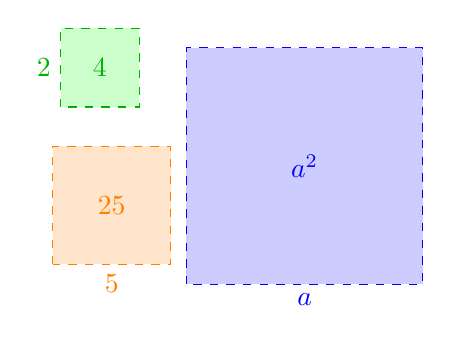
\begin{tikzpicture}
            \fill[blue!20,draw=blue, dashed] (0,0) -- (0,3) -- (3,3) -- (3,0) -- node[below,blue] {$a$} cycle;
            \fill[orange!20,draw=orange, dashed] (-1.7,0.25) -- (-1.7,1.75) -- (-0.2,1.75) -- (-0.2,0.25) -- node[below,orange] {$5$} cycle;
            \fill[green!20,draw=green!70!black, dashed] (-1.6,2.25) -- node[left,green!70!black] {$2$} (-1.6,3.25) -- (-0.6,3.25) -- (-0.6,2.25) -- cycle;
            \node[blue] at (1.5,1.5) {$a^2$};
            \node[orange] at (-0.95,1) {$25$};
            \node[green!70!black] at (-1.1,2.75) {$4$};
        \end{tikzpicture}
    }
    %\parpic[r]{
        
    %}
    \picskip{8}
    Der Flächeninhalt eines Quadrats mit der Seitenlänge $a$ ist $a^2$. Die Variable $a$ bezeichnet hier die Seitenlänge, wird also als Platzhalter verwendet. Sie wird durch eine konkrete Zahl ersetzt, sobald ein konkreter Flächeninhalt ausgerechnet werden soll -- etwa des orangefarbenen Quadrats mit der Seitenlänge 5. Um den Flächeninhalt für ein bestimmtes Quadrat zu berechnen, musst du in der Formel das $a$ durch die Seitenlänge deines Quadrats ersetzen und dann alles ausrechnen.
    
    Hat das Quadrat beispielsweise die Seitenlänge $5$, dann ist also $a=5$ und der Flächeninhalt ist laut Formel $5^2=25$. Außerdem hat das grüne Quadrat den Flächeninhalt 4 -- man ersetzt erneut in der Formel $a^2$ für den Flächeninhalt das $a$, erhält $2^2$ und somit den Flächeninhalt.
\end{example}

Formeln wie die des Flächeninhalts von Quadraten sollen zunächst einmal allgemeingültig sein. Sie sollen nicht für bestimmte Werte aufgeschrieben werden, sondern so, dass man sie allgemein für beliebige Werte anwenden kann.

Mit anderen Worten: Wir verwenden Variablen, wenn wir aus irgendeinem Grund noch nicht wissen, mit welcher bestimmten Zahl wir es zu tun haben. Das kann mehrere Gründe haben:

\begin{enumerate}[label=(\arabic*)]
    \item Beim Aufschreiben einer \emph{allgemeinen Formel} möchtest du eine Regel aufschreiben, die für beliebige Zahlen gilt. Erst beim Anwenden der Formel steht die Zahl, die du für die Variable einsetzen musst, fest.
    \item Du möchtest Rechnungen aufschreiben, in denen ein bestimmter Wert verwendet wird, den du noch nicht kennst. Diesen Wert kannst du in deinen Formeln durch eine Variable ersetzen, die in diesem Fall auch \emph{Unbekannte} genannt wird, weil ihr Wert unbekannt ist.
\end{enumerate}

Die erste Anwendung von Variablen, nämlich zum Aufschreiben von Formeln, ist dir schon häufiger begegnet (etwa bei der Formel des Flächeninhalts von Quadraten). Wenn eine Variable in dieser Weise als Platzhalter für einen konstanten Wert eingesetzt wird, heißt sie \textbf{Parameter}. In ihrer zweiten Funktion, nämlich als \textbf{Unbekannte}, hast du Variablen bisher noch nicht direkt erlebt. Du kannst dir das wie der Kasten in einer Aufgabe wie
\[17-\Box=11\] 
vorstellen. Hier möchtest du wissen, welche Zahl in den Kasten gehört, damit die Rechnung stimmt. Der Wert des Kastens ist in diesem Beispiel die \emph{Unbekannte}. Ziel einer Rechnung mit einer Unbekannten ist es, den Wert der Unbekannten zu bestimmen. Dass du einen Wert bestimmen möchtest, wenn du bestimmte Informationen über ihn hast, ist ein Problem, das dir in der Praxs oft begegnet. Wir schauen uns im folgenden Beispiel an, wie so ein Problem aussehen kann.

\begin{example}
    \parpic[r]{
        \begin{tikzpicture}[scale=0.9]
            \node (germay) at (0,5.5) {
\includegraphics[height=4cm]{images/Deutschland.pdf}};
            \draw[fill=green!80!black] (-3,0) -- ++ (0:2) arc [start angle=180, end angle=108, radius=1] -- ++ (108:2) arc [start angle=108, end angle=180, radius=3];
            \draw[fill=green!50!black] (1,0) -- ++ (0:2) arc [start angle=0, end angle=67.5, radius=3] -- ++ (247.5:2) arc [start angle=67.5, end angle=0, radius=1];
            \draw[fill=green!65!black] (108:1) arc [start angle=108, end angle=67.5, radius=1] -- ++ (67.5:2) arc [start angle=67.5, end angle=108, radius=3] -- ++ (-72:2);
            \draw[fill=white] (180:1) arc [start angle=180, end angle=0, radius=1] -- cycle;
            \node at (90:0.3) {\small 48 Teams};
            \node[text width=2cm, align=center] at (30:2) {Süd-deutsch-land};
            \node[text width=2cm, align=center] at (84:2) {Mittel-deutsch-land};
            \node[text width=2cm, align=center] at (145:2) {Nord-deutsch-land};
            \draw[thick, white, fill=green!65!black] (-0.2,5) -- (0.2,5) -- (0.2,3.2) -- (0,2.8) -- (-0.2,3.2) -- cycle;
            \draw[thick, white, fill=green!50!black] (0.6,4) arc [start angle=90, end angle=-20, radius=1.2] -- ++ (-83.43:0.447) -- ++ (43.43:0.447) arc [start angle=-20, end angle=90, radius=1.6] -- cycle;
            \draw[thick, white, fill=green!80!black] (-0.75,6) arc [start angle=120, end angle=200, radius=3.3] -- ++ (263.43:0.447) -- ++ (136.57:0.447) arc [start angle=200, end angle=120, radius=3.7] -- cycle;
        \end{tikzpicture}
    }
    
    An einer Deutschen Meisterschaft im Handball sollen insgesamt 48 Mannschaften teilnehmen. Die Regionen Norddeutschland, Mitteldeutschland und Süddeutschland erhalten dafür jeweils eine bestimmte Anzahl an Qualifikationsplätzen. Weil es in Norddeutschland doppelt so viele Mannschaften wie in Süddeutschland gibt, soll es auch doppelt so viele Qualifikationsplätze für Norddeutschland geben wie für Süddeutschland. Mitteldeutschland hat sogar dreimal so viele Mannschaften wie Süddeutschland und soll deswegen sogar dreimal so viele Qualifikationsplätze bekommen.
    
    \picskip{2}
    Nun stellt sich die Frage, wie viele Qualifikationsplätze Südddeutschland beispielsweise erhält. Wir wissen nun, dass alle Regionen zusammen 48 Plätze erhalten, also
    \[\textsc{Plätze Süden}+\textsc{Plätze Mitte}+\textsc{Plätze Norden}=48.\]
    Diesen Zusammenhang können wir direkt aus den gegebenen Informationen aufschreiben und er wird uns im Folgenden helfen, das Problem zu lösen. Später in diesem Kapitel werden wir diese Gleichung lösen und bestimmen, wie viele Qualifikationsplätze welche Region verteilen darf.
\end{example}

Du hast im Beispiel gesehen, dass die Informationen, die dir zur Verfügung standen, direkt in die mathematische Sprache übersetzt wurden. Vielleicht wirkt es seltsam, klar verständliche Informationen in Formeln zu übersetzen, die möglicherweise viel verwirrender als der ursprüngliche Text aussehen. Allerdings ist dies sehr viel kompakter und übersichtlicher als wenn du dauerhaft mit dem Text arbeiten würdest. Formeln erlauben es, sich auf das Wesentliche zu konzentrieren und somit nicht von Nebensächlichkeiten ablenken zu lassen.

Um einen Term aufzuschreiben, in dem ein Wert vorkommt, der dir unbekannt ist, wurden im Beispiel die Variablen \textsc{Plätze Süden}, \textsc{Plätze Mitte} und \textsc{Plätze Norden} verwendet. So kannst du den Term erstmal direkt aufschreiben und dir hinterher darüber Gedanken machen, was \textsc{Plätze Süden}, \textsc{Plätze Mitte} und \textsc{Plätze Norden} für Werte annehmen müssen. Wir geben unseren Unbekannten im Folgenden jedoch lieber Namen, die sich nicht nur für dieses eine Beispiel eignen, sondern die allgemein verwendet werden können, nämlich $x, y$ und $z$.

Wenn es darum geht, den Wert einer Unbekannten zu ermitteln, werden dafür irgendwelche Informationen über die Unbekannte benötigt -- in der Regel bekommst du diese Informationen durch eine \textbf{Gleichung}, in der die Unbekannte vorkommt.

Eine Gleichung sagt über zwei verschiedene Terme aus, dass sie gleich sind, also den gleichen Wert haben, wenn man sie ausrechnet. Beispielsweise ist $2+2=4$ eine Gleichung, denn sie sagt aus, dass $2+2$ das gleiche ist wie $4$. Deswegen liest man diese Gleichung auch als \enquote{$2+2$ \emph{ist gleich} $4$}.

\parpic[r]{
    \begin{linearEquation}
        %Füllung linke Waagschale
        \fill (-0.95,0.25) -- (-0.55,0.25) -- (-0.6,0.6) -- (-0.9,0.6) -- cycle;
        \draw[line width=0.75mm] (-0.75,0.66) circle[radius=0.06cm];
        \node[white] at (-0.75,0.42) {$2$};
        \fill (-1.45,0.25) -- (-1.05,0.25) -- (-1.1,0.6) -- (-1.4,0.6) -- cycle;
        \draw[line width=0.75mm] (-1.25,0.66) circle[radius=0.06cm];
        \node[white] at (-1.25,0.42) {$2$};
        %Füllung rechte Waagschale
        \fill (0.75,0.25) -- (1.25,0.25) -- (1.2,0.65) -- (0.8,0.65) -- cycle;
        \draw[line width=0.75mm] (1,0.71) circle[radius=0.06cm];
        \node[white] at (1,0.45) {$4$};
    \end{linearEquation}
}
Bei einer Gleichung ist es wichtig, dass links und rechts vom Gleichheitszeichen zwei gleichwertige Terme stehen. $2+2=4$ ist eine der einfachsten Gleichungen, die man sich vorstellen kann. Die Balkenwaage soll zeigen, dass der linke Teil der Gleichung (nämlich $2+2$, linke Waageschale) den gleichen Wert wie der rechte Teil der Gleichung (nämlich $4$, rechte Waagschale) haben muss. Die Balkenwaage befindet sich im Gleichgewicht.

Es kann manchmal helfen, sich Gleichungen als eine Balkenwaage vorzustellen, auf deren Waagschalen jeweils die Teile links und rechts vom Gleichheitszeichen liegen. Dadurch wird nämlich klar, dass links und rechts vom Gleichheitszeichen immer dasselbe stehen muss, damit die Waage im Gleichgewicht ist. Später in diesem Kapitel werden wir Gleichungen modifizieren und müssen dabei immer darauf achten, dass trotzdem noch dasselbe auf beiden Seiten steht -- oder, anschaulich gesprochen, die Balkenwaage nicht aus dem Gleichgewicht gerät.

\begin{example}
    \begin{center}
        \begin{linearEquation}
            %Füllung linke Waagschale
            \fill (-1.25,0.25) -- (-0.75,0.25) -- (-0.8,0.6) -- (-1.2,0.6) -- cycle;
            \draw[line width=0.75mm] (-1,0.66) circle[radius=0.06cm];
            \node[white] at (-1,0.42) {$20$};
            %Füllung rechte Waagschale
            \fill (0.75,0.25) -- (1.25,0.25) -- (1.2,0.65) -- (0.8,0.65) -- cycle;
            \draw[line width=0.75mm] (1,0.71) circle[radius=0.06cm];
            \node[white] at (1,0.45) {$20$};
        \end{linearEquation}
        \begin{linearEquation}
            %Füllung linke Waagschale
            \fill (-0.95,0.25) -- (-0.55,0.25) -- (-0.6,0.6) -- (-0.9,0.6) -- cycle;
            \draw[line width=0.75mm] (-0.75,0.66) circle[radius=0.06cm];
            \node[white] at (-0.75,0.42) {$5$};
            \fill (-1.45,0.25) -- (-1.05,0.25) -- (-1.1,0.6) -- (-1.4,0.6) -- cycle;
            \draw[line width=0.75mm] (-1.25,0.66) circle[radius=0.06cm];
            \node[white] at (-1.25,0.42) {$15$};
            %Füllung rechte Waagschale
            \fill (0.75,0.25) -- (1.25,0.25) -- (1.2,0.65) -- (0.8,0.65) -- cycle;
            \draw[line width=0.75mm] (1,0.71) circle[radius=0.06cm];
            \node[white] at (1,0.45) {$20$};
        \end{linearEquation}
    \end{center}
    Die linke Balkenwaage, bei der auf beiden Seiten das gleiche Gewicht liegt, ist im Gleichgewicht. Sie stellt die Gleichung $20=20$ dar. Das Gewicht stellt auf der Waage jeweils die Zahl links bzw. rechts vom Gleichheitszeichen dar.
    
    Die Rechnung $5+15=20$ ist ebenfalls eine Gleichung (zu sehen auf der rechten Balkenwaage). Ebenso wie bei jeder anderen Rechenaufgabe mit zugehörigem Ergebnis lässt sich hier beobachten, dass auf der linken Seite (also links vom $=$) derselbe Wert steht wie rechts -- nur auf mehrere Gewichte aufgeteilt. Letztendlich könntest du den Teil auf der linken Seite einfach ausrechnen, um zu sehen, dass du dort stattdessen auch ein einzelnes Gewicht mit dem Wert 20 hinlegen könntest.
\end{example}

Wenn bei einer Gleichung nur Zahlen vorkommen (also keine Variablen), dann kannst du dir diese einfach als beschriftete Gewichte auf den Waagschalen einer Balkenwaage vorstellen. In diesem Kapitel interessieren wir uns allerdings vor allem für Gleichungen, in denen Unbekannte vorkommen. Die Werte dieser Unbekannten sollen ermittelt werden. Das kannst du dir so vorstellen, dass du das Gewicht eines Gegenstandes ermitteln möchtest, der auf der Waage liegt.
 
\begin{example}
    \parpic[r]{
        \begin{linearEquation}
            %Füllung linke Waagschale
            \fill (-0.95,0.25) -- (-0.55,0.25) -- (-0.6,0.6) -- (-0.9,0.6) -- cycle;
            \draw[line width=0.75mm] (-0.75,0.66) circle[radius=0.06cm];
            \node[white] at (-0.75,0.42) {$3$};
            \node[white,marble,inner sep=.2cm] at (-1.2,0.35) {};
            %Füllung rechte Waagschale
            \fill (0.75,0.25) -- (1.25,0.25) -- (1.2,0.65) -- (0.8,0.65) -- cycle;
            \draw[line width=0.75mm] (1,0.71) circle[radius=0.06cm];
            \node[white] at (1,0.45) {$16$};
        \end{linearEquation}
    }
    
    Auf der rechts abgebildeten Balkenwaage liegt neben Gewichten eine blaue Kugel, die vollkommen unbeschriftet ist. Damit wir wissen, wie viel die Kugel wiegt, müsste sie allein auf der linken Seite liegen.
    
    \picskip{3}
    Insgesamt steht auf der linken Seite also ein unbekanntes Gewicht sowie ein Gewicht mit der Beschriftung 3. Das unbekannte Gewicht ist eine \emph{Unbekannte}, also eine Variable. Es ist üblich, Unbekannte mit dem Buchstaben $x$ zu bezeichnen. Links beträgt das Gesamtgewicht also $x+3$. Das Gewicht, das dort liegt, ist nämlich die Summe des beschrifteten Gewichts (also 3) und des Gewichts der Kugel (also $x$).
    
    Auf der rechten Seite ist die Situation einfacher: Hier ist das Gewicht $16$. Damit haben wir hier die Gleichung $x+3=16$. Damit die Waage im Gleichgewicht ist, muss $x+3$ also denselben Wert haben wie 16. Um herauszufinden, wie viel die Kugel wiegt, musst du dir für die Aufgabe 
    \[\Box+3=16\] 
    überlegen, welcher Wert in die Box kommt. Du wirst später sehen, dass solche Aufgaben manchmal schwierig zu lösen sind und dass es auch anders möglich ist, den Wert von $x$ zu ermitteln.
\end{example}

Um herauszufinden, welchen Wert eine Unbekannte haben muss, damit die Gleichung gilt (also auf beiden Seiten wirklich denselben Wert annimmt), musst du wie auf den letzten Seiten erklärt einen Wert finden, durch den du $x$ in der Gleichung überall ersetzen kannst. Möchtest du die Gleichung
\[\Box+65-3\cdot(\Box+2)=4\cdot \Box-103\]
lösen, also herausfinden, welcher Wert in die Box gehört, dann ist es manchmal nicht sinnvoll möglich, den Wert schnell durch Hinsehen zu bestimmen. Du müsstest in der obigen Gleichung beispielsweise überall den Wert 27 einsetzen (und das ist kein Wert, den man gern durch Ausprobieren suchen möchte). Wir entwickeln deshalb in diesem Kapitel Methoden, um diese Aufgaben auch zu lösen, wenn sie wesentlich komplizierter sind.

\end{document}
